\documentclass{article}

\usepackage[utf8]{inputenc}
\usepackage[T1]{fontenc}
\usepackage{polski}
\usepackage{indentfirst}
\usepackage{lastpage}
\usepackage{natbib}
\usepackage{graphicx} 
\usepackage{sidecap}
\usepackage{wrapfig}
\usepackage{subfig}
\usepackage{caption}

\captionsetup[figure]{name={Rysunek}}

\usepackage{fancyhdr}
\pagestyle{fancy}
\fancyhf{}
\rhead{A. Malinowski, F. Wysocki, B.Zakrzewski}
\rfoot{Strona \thepage \hspace{1pt} z \pageref{LastPage}}
\lhead{Spis treści}
\title{Specyfikacja funkcjonalna projektu pt. \\ ,,Patients Transport Center''}
\author{}
\date{}

\begin{document}
\maketitle

\begin{flushright}
\par
\vfill
\par
{\fontsize{11}{11}\selectfont
    Wykonali: Antoni Malinowski, Franciszek Wysocki, Bartosz Zakrzewski

    Sprawdzający: mgr inż. Paweł Zawadzki

    Data: 17-12-2020
}
\end{flushright}
\thispagestyle{empty}

\newpage

\tableofcontents

\newpage

\section{Cel dokumentu}
{\fontsize{12}{12}\selectfont
Celem dokumentu jest przedstawienie funkcjonalności programu, który zarządza transportem pacjentów do szpitali.

Zostanie w nim zaprezentowane w jaki sposób aplikacja powinna być uruchamiana, jak mają wyglądać pliki wejściowe i jak będzie wyglądać graficzny interfejs użytkownika.

Zostanie opisane jak zachowa się program w sytuacjach niepożądanych i co możemy do takich sytuacji zaliczyć.
}
\lhead{Cel dokumentu i projektu}

\section{Cel projektu}
{\fontsize{12}{12}\selectfont
Celem projektu jest symulacja w jaki sposób pacjenci mają być przewożeni do najbliższych szpitali. 
Program określi:
\begin{itemize}
    \item czy pacjent znajduje się na terenie obsługiwanym przez karetki pogotowia;
    \item który szpital jest najbliższy;
    \item czy są wolne łóżka w szpitalu - jeżeli nie, to przetransportuje pacjenta do kolejnego najbliższego szpitala.
\end{itemize}
}

\clearpage

\lhead{Scenariusz uruchomienia}

\section{Scenariusz uruchomienia}
{\fontsize{12}{12}\selectfont
\begin{enumerate}
    \item Użytkownik uruchamia aplikację. \\
    Pierwszy sposób uruchomienia:
    \begin{enumerate}
        \item Użytkownik uruchamia aplikację ,,patients-transport-center.jar” poprzez dwukrotne kliknięcie na jej ikonę lewym przyciskiem myszy;
        \item Użytkownik ustawia wstępną konfigurację (załącza ,,plik z mapą'' i ,,plik z pacjentami'').
    \end{enumerate}
    Drugi sposób uruchomienia:
    \begin{enumerate}
        \item Użytkownik uruchamia program z poziomu terminala za pomocą: 
            \begin{center}
                \texttt{java -jar patients-transport-center.jar} 
            \end{center}
            
        \item Użytkownik może podać nazwę pliku z obiektami, szpitalami i drogami oraz nazwę pliku z pacjentami, poprzez flagi ,,-h'' i ,,-p'':
        
        \begin{center}
                \texttt{java -jar patients-transport-center.jar \\}
                \texttt{-h nazwa-pliku-ze-szpitalami-obiektami-i-drogami \\ 
                -p nazwa-pliku-z-pacjentami}
        \end{center}
        
        Jeżeli jakaś flaga nie zostanie podana, użytkownik będzie musiał wczytać pliki z poziomu interfejsu użytkownika.
    \end{enumerate}
    
    \item Użytkownik uruchamia symulację, w której na bieżąco obliczane są optymalne rozwiązania dla transportu pacjentów z pliku wejściowego;
    \item Użytkownik może wstawić kolejnego pacjenta na mapie za pomocą prawego przycisku myszki lub w panelu zarządzania;
    \item Użytkownik może przyspieszyć/spowolnić symulację w panelu zarządzania;
    \item Użytkownik może zmienić plik z mapą/listą nowych pacjentów w panelu zarządzania;
    \item Użytkownik może odczytać informacje o danym obiekcie naciskając na niego lewym przyciskiem myszki.
\end{enumerate}

    \clearpage
    Wizualizacja aplikacji stworzona za pomocą programu GIMP 2:
    \begin{figure} [hbt!]
        \centering
        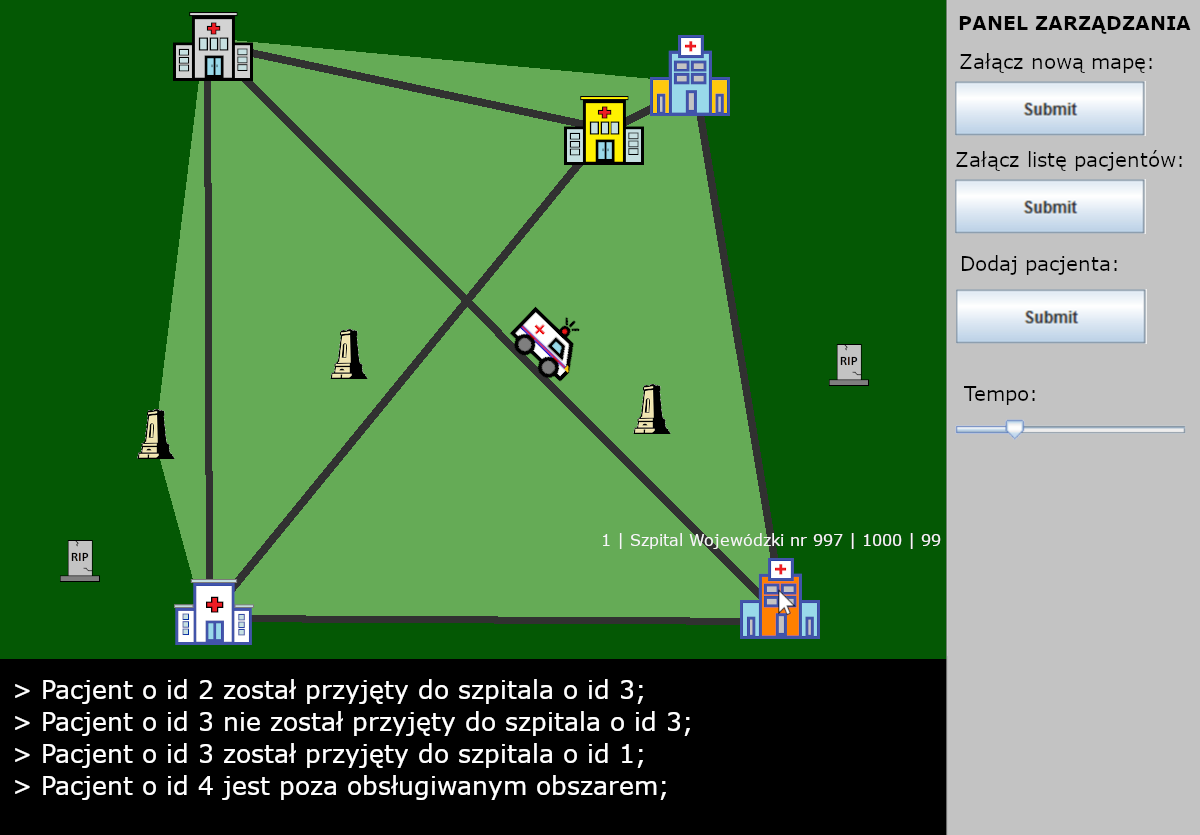
\includegraphics[width=13cm]{images/mapa_panele.png}
      \captionof{figure}{Wygląd programu}
    \end{figure}
    
Mapa będzie reprezentowała obiekty zgodnie z ich położeniem w układzie współrzędnych. 
Pod nią znajdować się będzie panel z wyświetlanymi komunikatami, a obok niej panel zarządzania. \\

Transport pacjentów będzie odbywać się ,,pacjent po pacjencie’’, aby czytelniej przedstawić symulację.
}

\clearpage

\lhead{Dane wejściowe}

\section{Opis danych wejściowych}
{\fontsize{12}{12}\selectfont

Program, jak już to wcześniej opisano w sekcji \textbf{Scenariusz uruchomienia},  wymagać będzie dostarczenia \textbf{2 plików wejściowych} (muszą być to plik tekstowe). 

\subsection{Plik pierwszy}
Pierwszy plik wejściowy będzie się składać z następujących \textbf{trzech sekcji}:
\begin{itemize}
    \item Szpitale (id | nazwa | wsp. x | wsp. y | liczba łóżek | liczba wolnych łóżek);
    \item Obiekty (id | nazwa | wsp. x | wsp. y);
    \item Drogi (id | id\_szpitala | id\_szpitala | odległość).
\end{itemize}

Nazwę każdej sekcji należy poprzedzić znakiem ,,\#''. \\
Każda sekcja musi zawierać wiersze,  w których zapisane będą surowe dane wykorzystywane przez program.  \\
Wiersze w poszczególnych sekcjach muszą posiadać odpowiednią strukturę, zdefiniowaną w nawiasie po nazwie sekcji.

    \begin{figure} [hbt!]
        \centering
        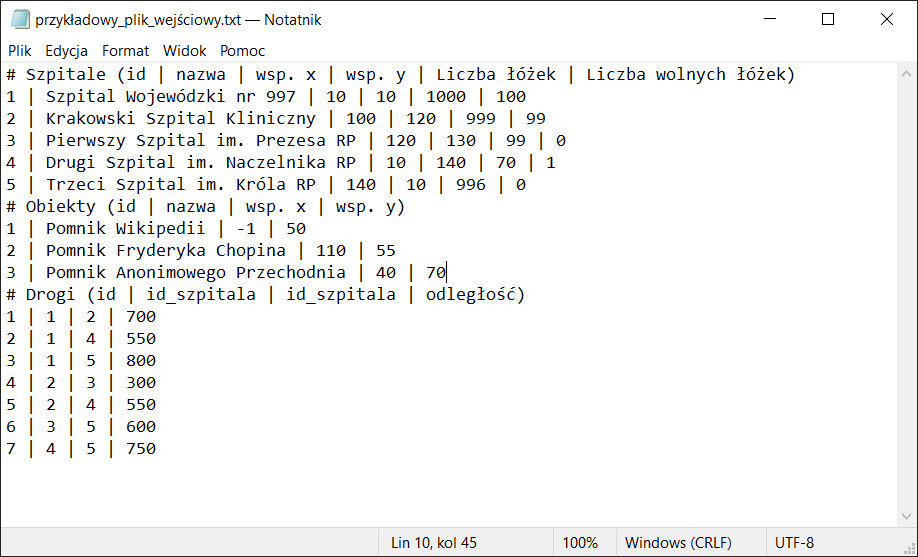
\includegraphics[width=14cm]{images/przykładowy_plik_wejściowy.PNG}
      \captionof{figure}{Przykładowy plik wejściowy}
    \end{figure}
    
\clearpage

\subsection{Plik drugi}
Drugi plik wejściowy to lista zawierająca \textbf{pacjentów i ich współrzędne}.
Pacjenci będą obsługiwani w kolejności w jakiej są w pliku. Po przetransportowaniu wszystkich pacjentów z pliku, zostaną po kolei transportowani pacjenci dodani z poziomu aplikacji.

W pliku ma znajdować się jedna sekcja:
\begin{itemize}
    \item Pacjenci (id | wsp. x | wsp.y).
\end{itemize}


Tak jak w przypadku pierwszego pliku, nazwa sekcji musi być poprzedzona znakiem ,,\#'', a wiersze muszą posiadać strukturę widoczną w nawiasach.

 \begin{figure} [hbt!]
        \centering
        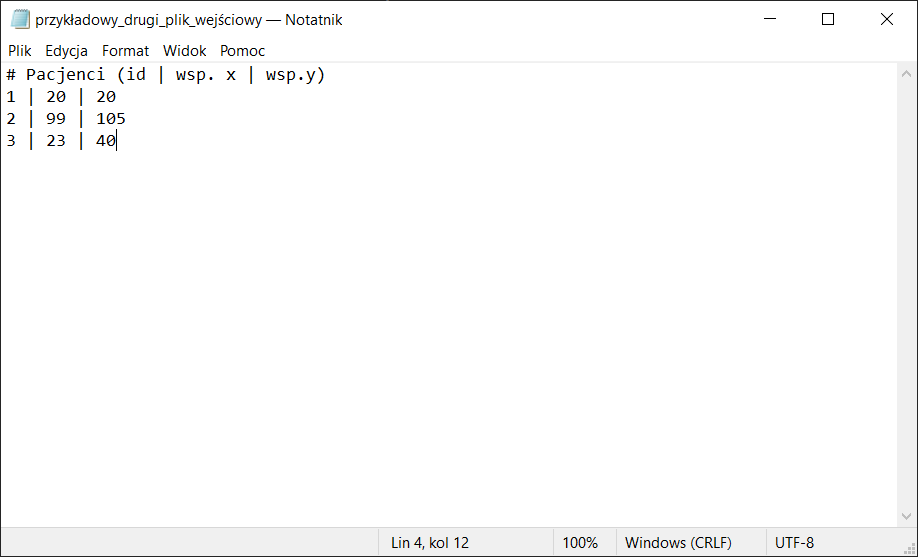
\includegraphics[width=15cm]{images/przykładowy_drugi_plik_wejściowyPNG.PNG}
      \captionof{figure}{Przykładowy drugi plik wejściowy}
    \end{figure}
    
\clearpage

\subsection{Struktura wierszy w sekcji}
Każdy wiersz niebędący nazwą sekcji musi posiadać strukturę określoną po nazwie sekcji, w której się znajduje. Opis struktury zawiera etykiety, które informują o tym, co reprezentować będą dane w poszczególnych polach wiersza. \\

W sekcji ,,\textbf{Szpitale}'' i ,,\textbf{Obiekty}'' w kolumnie ,,\textbf{nazwa}'' (w kolejnych wierszach) musimy wpisać słowo (nazwa może być kilku członowa, ale nie może zawierać znaku ,, | ''). \\ 

Dla reszty pól, w wierszu należy wpisać \textbf{liczbę całkowitą} większą bądź równą 0 (wyjątkiem są tu pola w kolumnach \textbf{wsp.x} i \textbf{wsp. y}, gdzie wartościami mogą być dowolne liczby całkowite). \\

Poszczególne wartości w wierszu muszą być oddzielone symbolem ,, | '' (spacja + znak strumienia + spacja). \\

\underline{Sytuacje niedopuszczalne}:
Sytuacje, dla których program nie będzie mógł poprawnie odczytać zawartości podanych plików wejściowych to:

\begin{itemize}
    \item niepoprawne odseparowanie od siebie wartości w poszczególnych wierszach;
    \item niepoprawna kolejność sekcji (np. zamiana miejscami sekcji szpitali z sekcją obiektów);
    \item brak znaku ,,\#'' przed nazwą sekcji;
    \item niepoprawnie podane wartości (liczby z wartością po przecinku, liczby całkowite mniejsze od zera dla pól innych niż wartości współrzędnych).
\end{itemize}

}

\clearpage

\lhead{Komunikaty o błędach}
\section{Komunikaty o błędach}
{\fontsize{12}{12}\selectfont

W razie wystąpienia błędu, wyświetli się komunikat w wyskakującym oknie (popup). Niektóre błędy będą zmuszały użytkownika do zakończenia działania aplikacji (np. brak obrazu karetki), inne będą wskazywały błąd i oczekiwały naprawy (np. błąd w pliku wejściowym). \\
   
Komunikaty będą pojawiały się między innymi podczas:
   \begin{itemize}
        \item błędnej walidacji pliku;
        \item nieodnalezienia pliku;
        \item nieodnalezienia obrazów/sprite’ów obiektów.
   \end{itemize}
   
}

\section{Źródła}
{\fontsize{12}{12}\selectfont
\begin{itemize}
    \item Przykładowe dane wejściowe przygotował mgr inż. Paweł Zawadzki;
    \item Rysunek poglądowy został stworzony za pomocą programów: GIMP 2, Paint, Paint 3D;
    \item Ten dokument został stworzony za pomocą strony overleaf.com.
\end{itemize}
}    

\end{document}
